\onecolumn\twocolumn
\section{Evaluation}
\label{sec:eval}

% These top level graphs are based on raw data and pick some select points.
% If you want to see the full tput-latency graphs, uncomment the section of graphs at the bottom

%%%%%%%%%%%%%%%%%%%%%%%%%%%%%%%%%%%%%%%%
%%%%%%%%%%%% Uniform fanout %%%%%%%%%%%%
%%%%%%%%%%%%%%%%%%%%%%%%%%%%%%%%%%%%%%%%
% Single shard p99 + p50
\begin{figure*}[!htb]
\centering
\subfloat[1 shard p99]{
  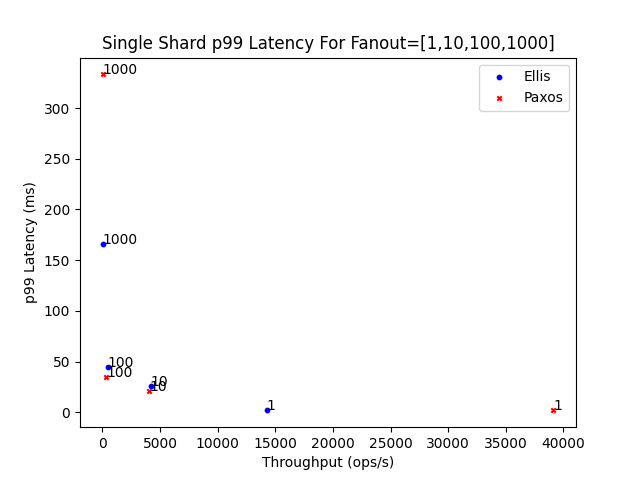
\includegraphics[scale=.6]{figs/1shardp99.png}
  \label{fig:1shardp99}
}
\subfloat[1 shard p50]{
  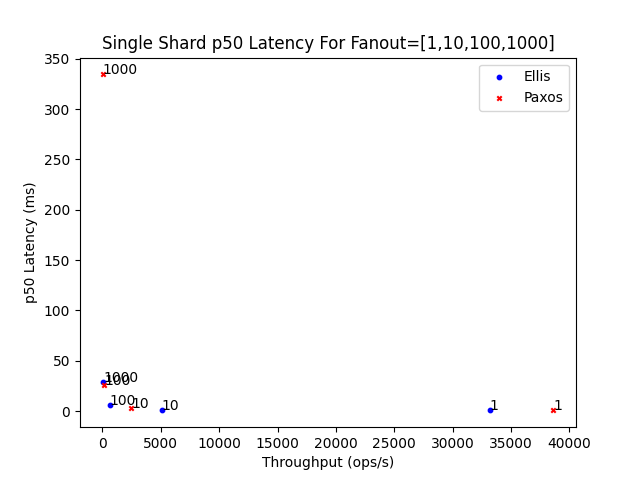
\includegraphics[scale=.6]{figs/1shardp50.png}
  \label{fig:1shardp50}
}
\hspace{0mm}
% 3 shards p99 + p50
\centering
\subfloat[3 shard p99]{
  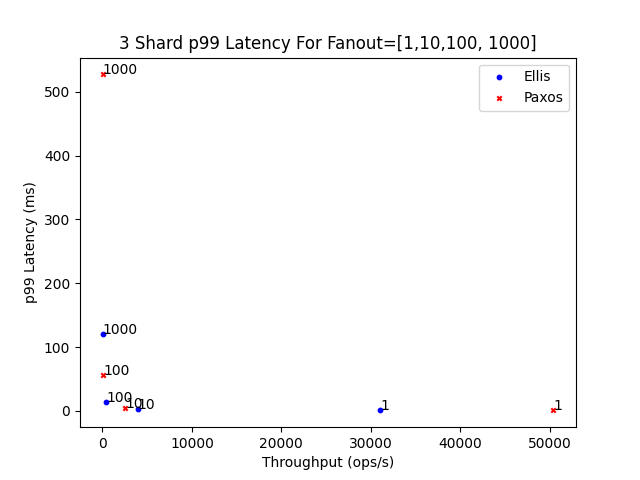
\includegraphics[scale=.6]{figs/3shardp99.png}
  \label{fig:3shardp99}
}
\subfloat[3 shard p50]{
  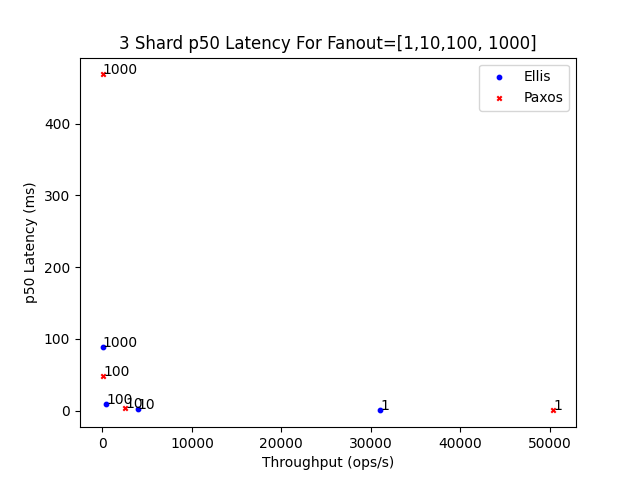
\includegraphics[scale=.6]{figs/3shardp50.png}
  \label{fig:3shardp50}
}
\hspace{0mm}
% 9 shards p99 + p50
\centering
\subfloat[9 shard p99]{
  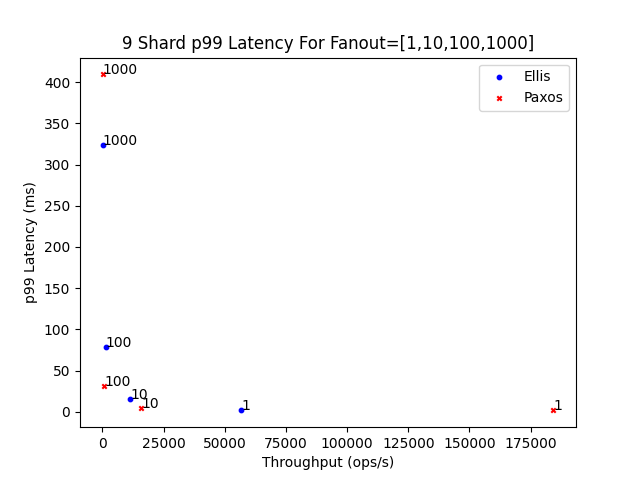
\includegraphics[scale=.6]{figs/9shardp99.png}
  \label{fig:9shardp99}
}
\subfloat[9 shard p50]{
  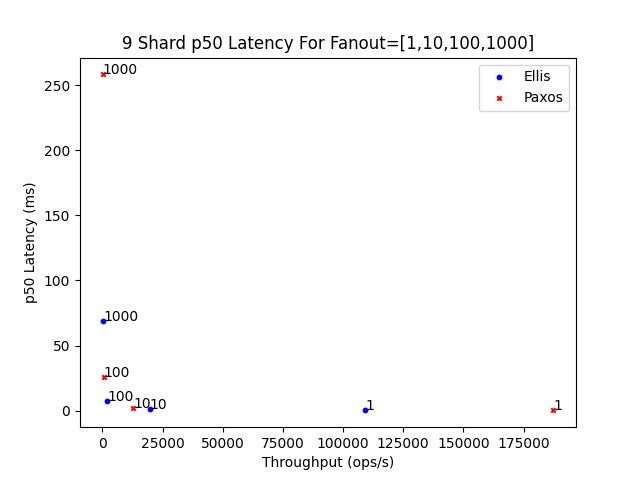
\includegraphics[scale=.6]{figs/9shardp50.png}
  \label{fig:9shardp50}
}
\caption{p99 and p50 for various shard settings.}
\end{figure*}

%%%%%%%%%%%%%%%%%%%%%%%%%%%%%%%%%%%%%%%%
%%%%%%%%%%%% 3 shard skew %%%%%%%%%%%%%%
%%%%%%%%%%%%%%%%%%%%%%%%%%%%%%%%%%%%%%%%
\begin{figure*}[!htb]
\centering
\subfloat[skew\xspace0.]{
  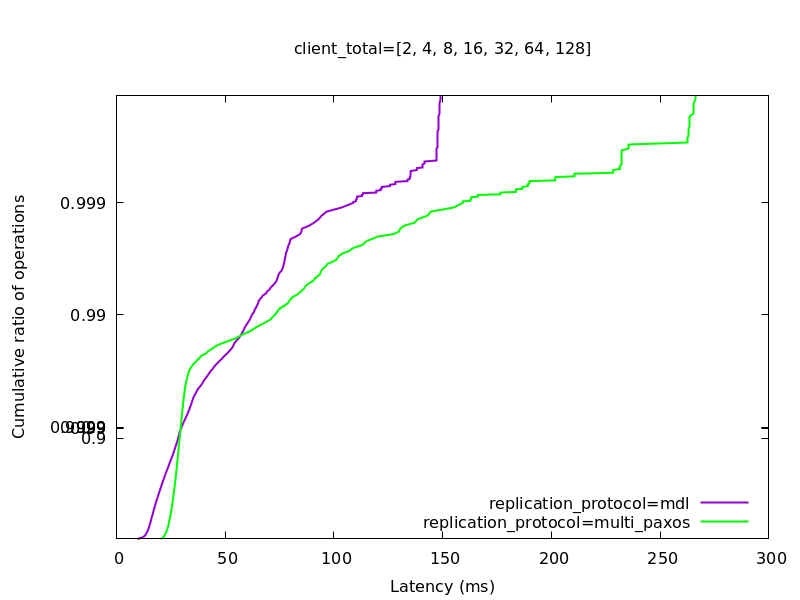
\includegraphics[scale=.1]{figs/3shards_fanout100_skew0.5_16client_CDF.png}
}
\subfloat[skew\xspace0.7]{
  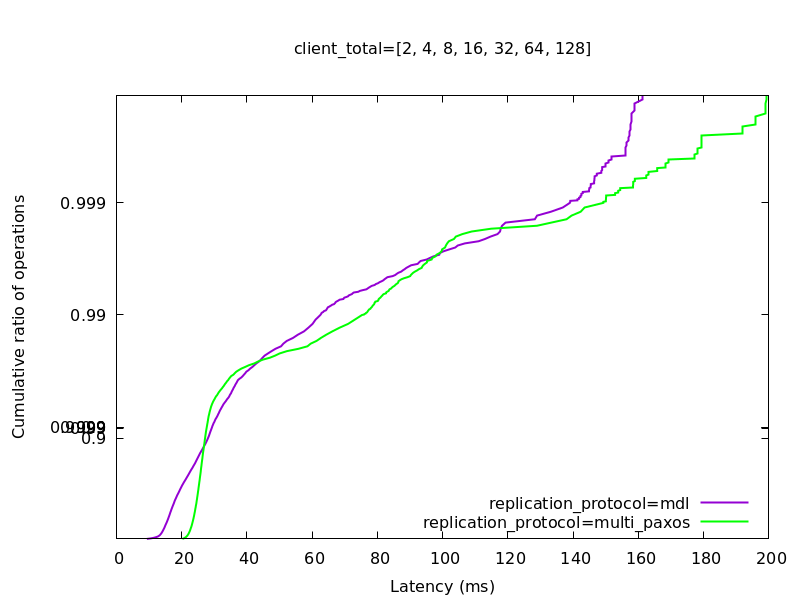
\includegraphics[scale=.1]{figs/3shards_fanout100_skew0.7_16client_CDF.png}
}
\subfloat[skew\xspace0.9]{
  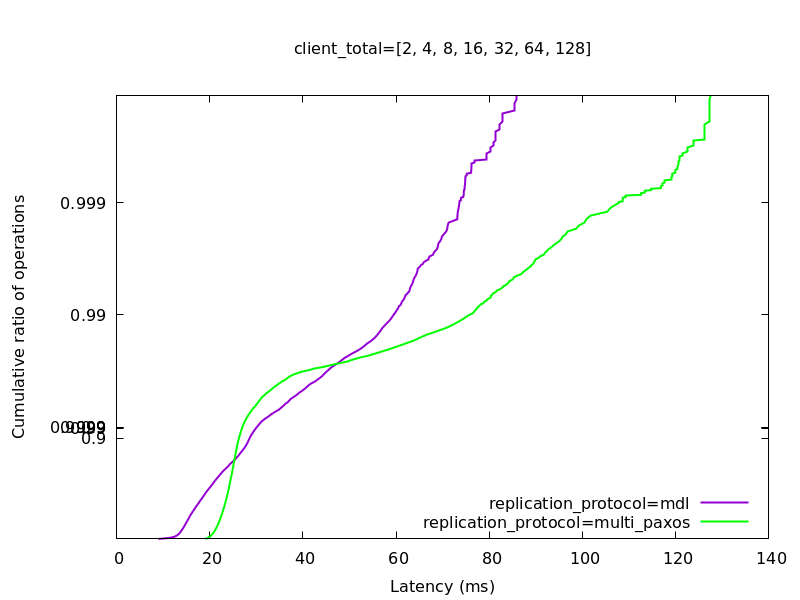
\includegraphics[scale=.1]{figs/3shards_fanout100_skew0.9_16client_CDF.png}
}
\subfloat[skew\xspace1.1]{
  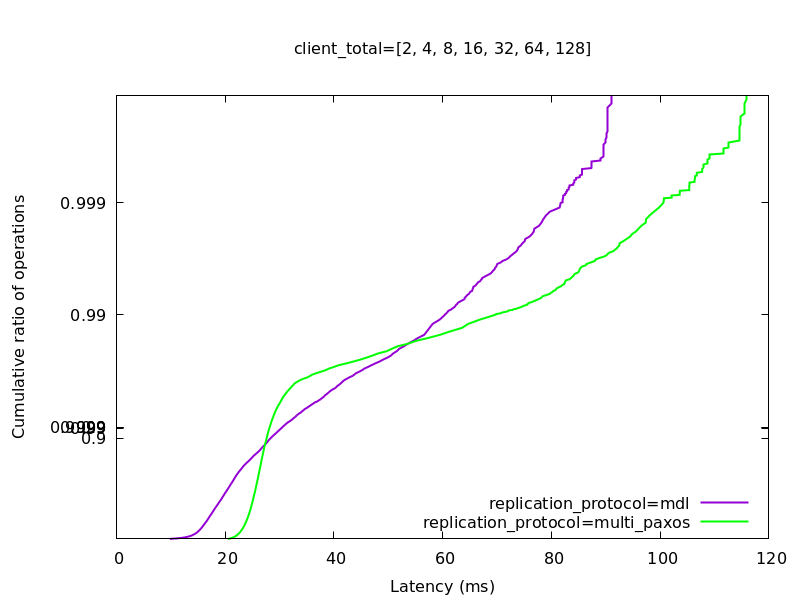
\includegraphics[scale=.1]{figs/3shards_fanout100_skew1.1_16client_CDF.png}
}
\subfloat[skew\xspace1.3]{
  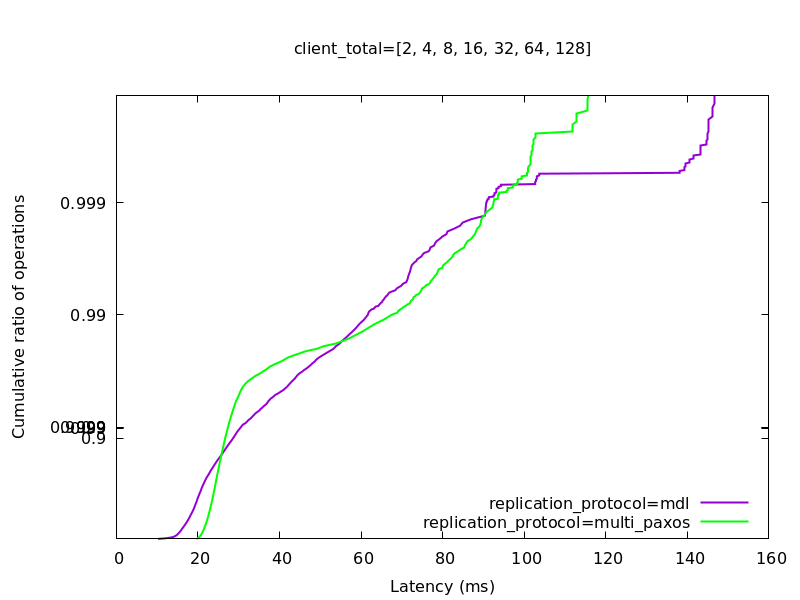
\includegraphics[scale=.1]{figs/3shards_fanout100_skew1.3_16client_CDF.png}
}
\caption{3 shard skew.}
\end{figure*}


%%%%%%%%%%%%%%%%%%%%%%%%%%%%%%%%%%%%%%%%
%%%%%%%%%%%% 9 shard skew %%%%%%%%%%%%%%
%%%%%%%%%%%%%%%%%%%%%%%%%%%%%%%%%%%%%%%%
\begin{figure*}[!htb]
\centering
\subfloat[skew\xspace0.5]{
  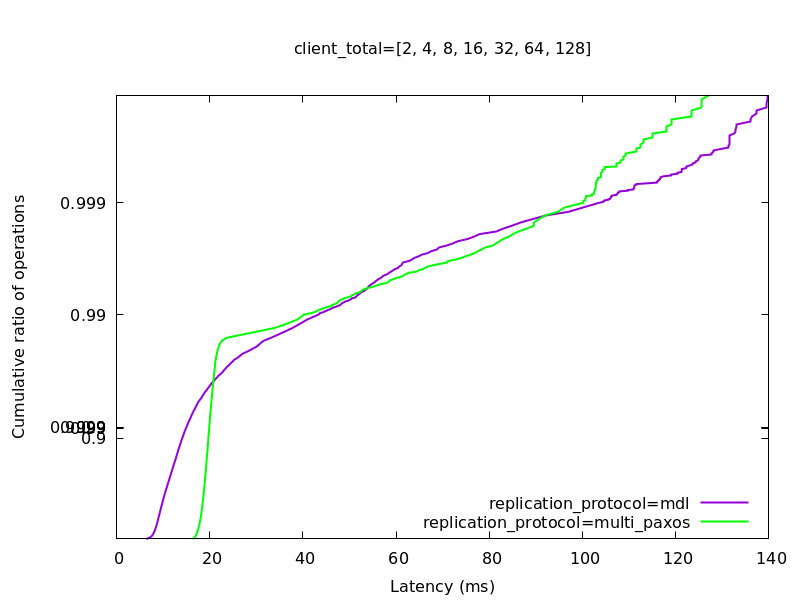
\includegraphics[scale=.1]{figs/9shards_fanout100_skew0.5_16client_CDF.png}
}
\subfloat[skew\xspace0.7]{
  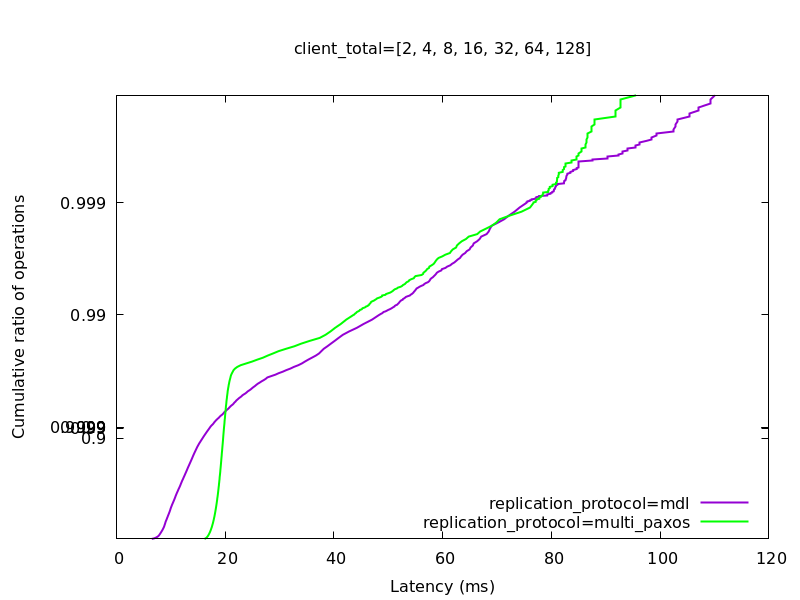
\includegraphics[scale=.1]{figs/9shards_fanout100_skew0.7_16client_CDF.png}
}
\subfloat[skew\xspace0.9]{
  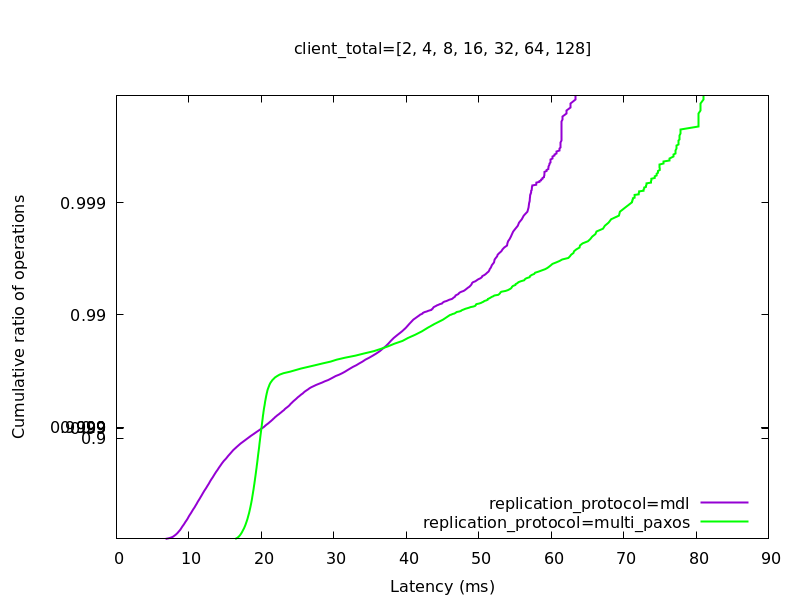
\includegraphics[scale=.1]{figs/9shards_fanout100_skew0.9_16client_CDF.png}
}
\subfloat[skew\xspace1.1]{
  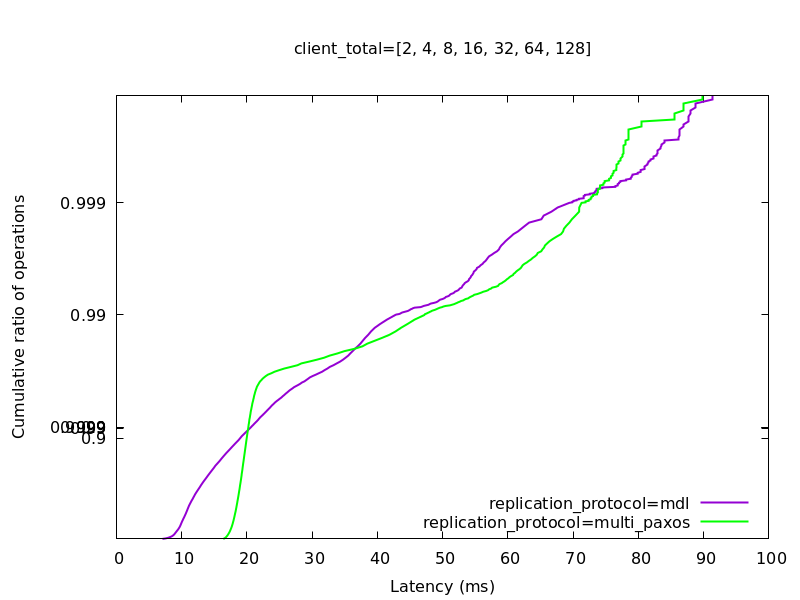
\includegraphics[scale=.1]{figs/9shards_fanout100_skew1.1_16client_CDF.png}
}
\subfloat[skew\xspace1.3]{
  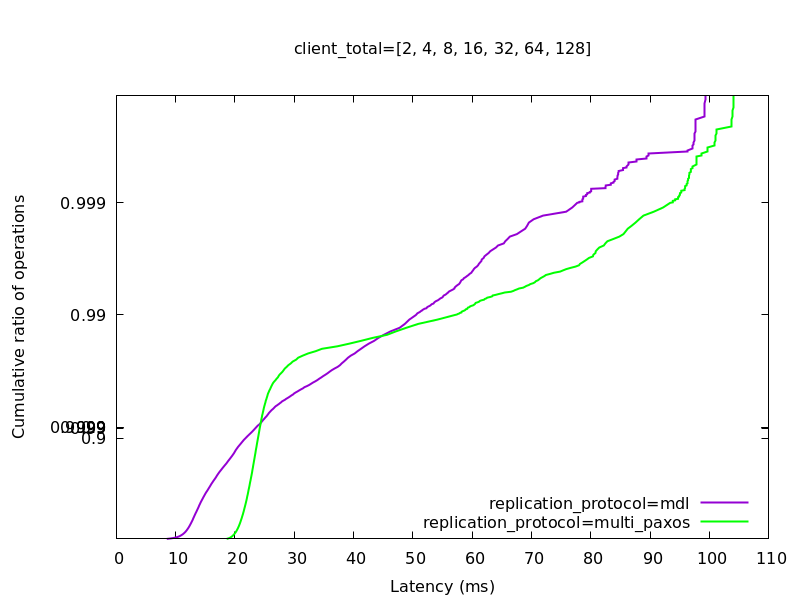
\includegraphics[scale=.1]{figs/9shards_fanout100_skew1.3_16client_CDF.png}
}
\caption{9 shard skew.}
\end{figure*}

%%%%%%%%%%%%%%%%%%%%%%%%%%%%%%%%%%%%%%%%%%%%%%%%%%%%%%%%%%%%%%%%%%%%%%%%%%%%%%%%%%%
%%%%%%%%%%%%%%%%%%%%%%%%%%%%%%%%%%%%%%%%%%%%%%%%%%%%%%%%%%%%%%%%%%%%%%%%%%%%%%%%%%%

%TODO
This section describes how we evaluate \system's performance handling requests from multi-dispatch clients compared to \mpaxos's performance handling requests from single-dispatch clients. 
Our focus is on measuring latency and throughput of application-level requests, since we aim to improve end-to-end latency for applications.
We also look at how \system scales from single-shard to multi-shard configurations, and how sensitive performance is to skewed workloads.
We show that our approach achieves improves end-to-end latency for application level-requests, and scales with the number of subrequests (fanout) issued per application request. 

\subsection{Experimental Set-up}
All experiments are conducted on Cloudlab's Utah platform ~\ref{}, using m510 machines. 
Our experimental setup consists of a 9-node cluster and 2 client machines. 
Each machine has 1 Intel Xeon-D processor with 8 physical cores running at 2 GHz with hyperthreading enabled, 64 GB of DDR4-2133 RAM, and a 10 Gb/s NIC. 
The roundtrip latency between all machines is around 150 $\mu$s, thus intershard, intrashard, and client-leader latencies are all equal. 
Each shard contains 3 replicas, all placed on different physical machines. For multi-sharded experiments we place shard leaders on different physical machines as well. 
We set the epoch length for \system to 1 ms.alev

\al{combine experimental set-up and client design. get rid of metrics, workload,
failures and replace with, approximately, one sentence each in the experimental
setup or eval intro}

\subsection{Client Design}
We evenly distribute client processes across the 2 client machines. Client processes submit application-level requests. Each application-level request submits $n$ system-level subrequests, where $n$ is equal to the fanout parameter for a given experiment. For single-dispatch clients interacting with \mpaxos, only a single system-level subrequest is in-flight at a time, the next subrequest is not issued until the response is received for the preceding subrequest. For multi-dispatch clients interacting with \system, all $n$ system-level subrequests are in-flight at the same time, each is submitted in order and does not wait until the response is received for the preceding subrequest.

Each client process is a closed-loop client that submits a single application-level request at a time. The next application-level request is not submitted until all subrequests return. 

In each experiment, we scale the number of clients issueing requests to both systems from 2 to 128 by factors of 2. It's worth noting that since multi-dispatch clients have $n$ requests in-flight at a time, while single-dispatch clients only have 1 request in-flight at a time, \system leaders have to deal with $n$ more requests than \mpaxos at any given time for the same number of clients, which is a disadvantage for our system.

%For a fair comparison between MDL and SDL, we keep the number of outstanding requests sent to each system the same. To achieve this, MDL uses a smaller number of clients $K$ with the specified number $N$ of outstanding requests per client, while SDL uses $K*N$ clients each with 1 outstanding request per client.

% \wl{How does keeping the overall number of requests the same mean the load is the same? We discussed this, you can explain this clearly: keep number of outstanding requests the same in both systems, for mdl this uses a smaller number of clients with the specified number of outstanding requests per client, for sdl its N clients with 1 outstanding request per client.}

\subsection{Metrics}
% perhaps we should look at p90
We report on both the p99 and p50 for application-request latency. 
We find p50 a useful metric to look at since our decision to evaluate application-level requests is already end-user facing. 

While we report p99, we do not find this metric representative of the average case latency that users should expect when interacting with \system. This could be due to a number of factors, such as the variability of each system-level request (which we do not focus on improving), the single-threaded implementation of our servers, and our use of Golang tickers to implement epochs.

\subsection{Workload}
We consider uniform and skewed key distributions to explore a more representative range of realistic workloads. For the latter, we generate keys according to a Zipfian distribution with varying skew values $\theta \in \{0.5, 0.7, 0.9, 1.1, 1.3\}$, and use a keyspace of size 1 million. 

We do not vary the request type at all, all workloads are 100\% writes, since neither our protocol nor basic Paxos implement op-type specific optimizations. 

\subsection{Failures}
We do not consider leader failover in this evaluation. Since failures are rare, and unavoidably degrade performance for most protocols, we only consider the normal mode of operation for \system and \mpaxos. Details about the failover specifics in the protocol can be found in ~\ref{sec:design}.

\subsection{Single-Shard}
In this section, we compare the end-to-end application request latency for \system and \mpaxos configured with a single shard. We consider uniform key distribution and vary the fanout parameter as $1$, $10$, $100$, and $1000$.

For each fanout value, we find the number of clients that saturates \system, and show the p99 and p50 latencies. We also show the p99 and p50 latencies for \mpaxos for the same number of clients we picked for \system. Note, this selection for number of clients does not always saturate \mpaxos.

Figures ~\ref{fig:1shardp99} and ~\ref{fig:1shardp50} show the throughput latency curves for ranging fanout values of application-level requests. In the single-shard setting, the expected improvement is most sensitive to our selection of epoch length, as well as the relationship between this value and leader-replica roundtrip latenciy. Idealistically, (1) concurrent requests arrive at the leader as soon as an epoch begins, (2) replicate at a majority in parallel, (3) immediately afterwards the epoch expires, (4) the final ordering roundtrip completes, and (5) the requests are executed. Realistically, requests might arrive halfway through an initial epoch, and therefore remain in the buffered log for an additional trailing epoch. Since our implementation uses an epoch value of 1ms, and the leader-replica latency is around 150$\mu$s, \system is unable to match \mpaxos until around fanout 10. %Moreover our golang implementation of timers...

While a protocol that provides \mdl could be optimized for a single-shard setting ~\ref{}, we did not change same multi-sharded protocol for a single shard, therefore we still issue coordination messages for each request which the leader must process. The coordination overhead on a single shard is somewhat smaller as compared to the multi-shard setting since there is no leader-to-leader latency. However, at higher fanouts, the leader is under higher load and must process a large log of buffered requests and each of their coordination messages. We notice a substantial improvement for latencies at fanouts $100$ and $1000$, approaching greater than 50\%. This improvement is attenuated by the processing of coordination overhead for each request.


\al{Is there \emph{any} coordination overhead? Again, be more crisp and
concrete. For example (not sure this is true): Because there is no (or virtually
no) coordination overhead in the single-shard setting, \protocol{}'s performance
is dictated primarily by the epoch length and the intra-shard latency. As a
result, with our epoch length of 10ms, \protocol{} lags behind \mpaxos{} until
fan-out reaches approximately the ratio of intra-shard latency and epoch length
(about 10x).}

\subsection{Multi-Shard}
\label{sec:shards}
In this section, we look at the application-level request latencies for 3-shard and 9-shard configurations, shown in figures ~\ref{fig:3shardp99} -- ~\ref{fig:9shardp50}.

We expect \system to approach a 50\% improvement compared to \mpaxos as fanout increases.
As described in section ~\ref{sec:design}, an application-level request of fanout $n$ induces $n-1$ 1-way intershard coordination messages, that must be serialized with predecessor fault-tolerance and coordination.
Because of this, we see the multi-shard performance degrade for even fanout $100$. 
Moreover, with an epoch selection of 1ms, the requests issued last in an application-level request induce extra epoch lengths of waiting for coordination to arrive from the first concurrent request issued.

We notice improvement at 9-shards, however, as the coordination overhead per leader substantially decreases. We expect an optimal configuration to consider selecting a number of shards that balances load per leader.

%TODO probably remove this paragraph... i don't think it's actually a "win"
Finally, we chose not to vary the amount of time between system-level subreqeusts issued for each application-level request, all subrequests are sent immediately for multi-dispatch clients. Because of this, the final request wait the full coordination and committment latencies of each request that precedes it. For multi-dispatch clients that asynchronously issue requests with some variable delay between each request, this delay can overlap with the committment and coordination of predecessors, allowing successive reqeusts to appear to be coordinated sooner.
%show the latency improves at 9 shards over range of fanouts
%explain why it's better, what's happening, what overhead we've introduced
%mention that p50 is better.

\subsection{Skew}
In this section, we look at how varying key skew impacts the multi-shard performance of \system.
Our graphs show various skew values for the 3-shard and 9-shard configurations. We look at CDFs for application-level requests with fanout 100 issued by 16 concurrent clients. 

Overall we don't see much of an impact of skew on end-to-end latency.

\begin{comment}
\subsection{MDL with Geo-rep in the Wide Area}
\label{sec:wide}
We show the e2e app. latency for varying inter-shard latency (which we call the wide area **this might be wrong terminology) and inter-replica latency (which we call geo-replication, also might be wrong terminology).

\subsection{Applications on MDL}
\label{sec:apps}

As described in prior sections, we built a tool to automatically transform applications built to interact with SDL backends to interact with MDL backends, maintaining external equivalence. In this section we select 3 representative applications, A1, A2, A3, and show that when transformed with our tool, all 3 see an improvement in e2e latency. We use DeathStar to benchmark the applications.

A1 is an application that ....

A2 is an application that ...

A3 is an application that ...

We expect transformed applications that have a large degree of data parallelism and are read heavy running on MDL backends to see the largest e2e latency improvements over their pre-transformed counterparts running on SDL backends.

Jeff is still looking for these applications at the moment -- it would be good to pick applications that are read heavy and some that are mixed. All should include varying degrees of data parallelism, to show how some improve after the transformation more than others.
\end{comment}


%%%%%%%%%%%%%%%%%%%%%%%%%%%%%%%%%%%%%%%%%%%%%%%%%%%%%%%%%%%%%%%%%%%%%%%%%%%%%%%%%%%
%%%%%%%%%%%%%%%%%%%%%%%%%%%%%%%%%%%%%%%%%%%%%%%%%%%%%%%%%%%%%%%%%%%%%%%%%%%%%%%%%%%
%%%%%%%%%%%%%%%%%%%%%%%%%%%%%%%%%%%%%%%%
%%%%%%%% 1 shard uniform p99 %%%%%%%%%%%
%%%%%%%%%%%%%%%%%%%%%%%%%%%%%%%%%%%%%%%%
%\begin{comment}
\begin{figure*}[!htb]
\centering
\subfloat[Fanout\xspace1]{
  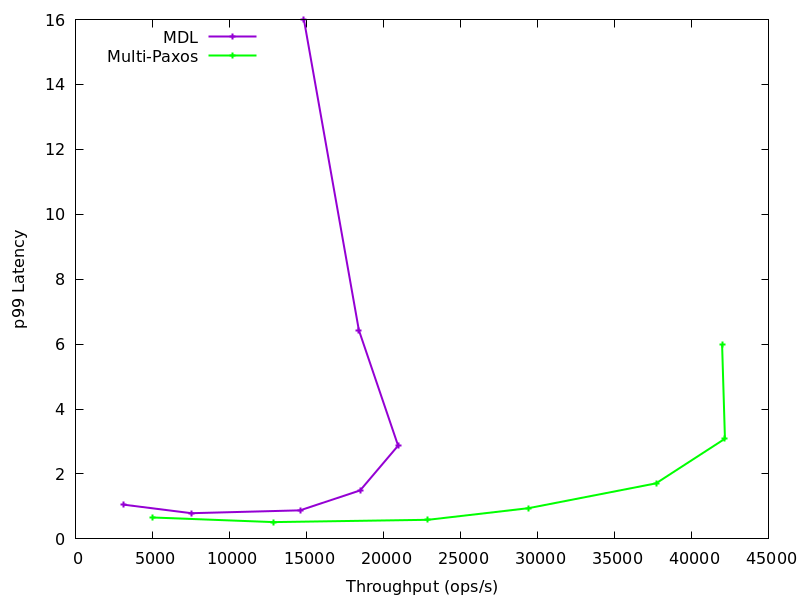
\includegraphics[scale=.15]{figs/1shard_fanout1_p99.png}
}
\subfloat[Fanout\xspace10]{
  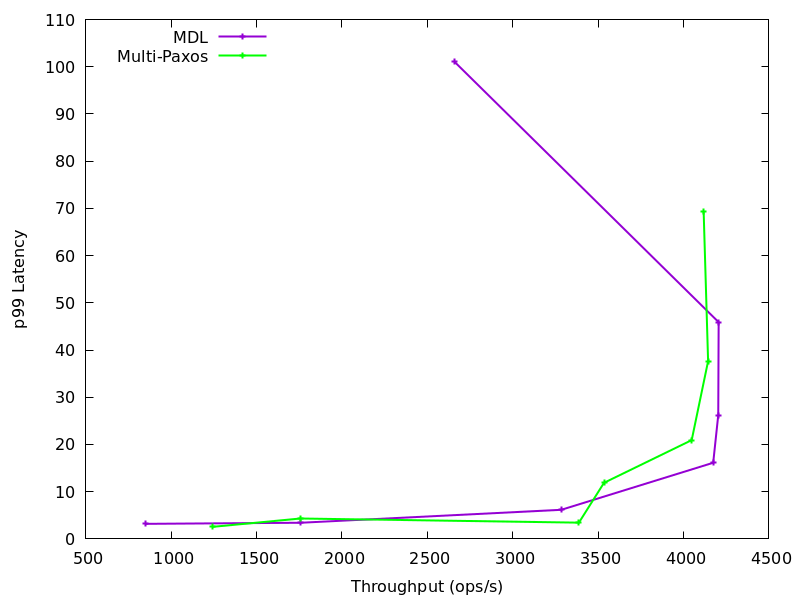
\includegraphics[scale=.15]{figs/1shard_fanout10_p99.png}
}
%\hspace{0mm}
\subfloat[Fanout\xspace100]{
  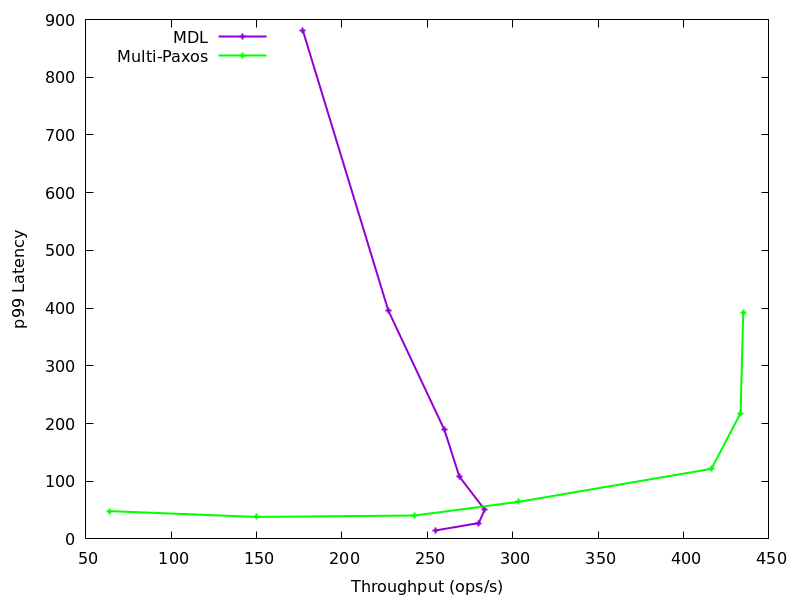
\includegraphics[scale=.15]{figs/1shard_fanout100_p99.png}
}
\subfloat[Fanout\xspace1000]{
  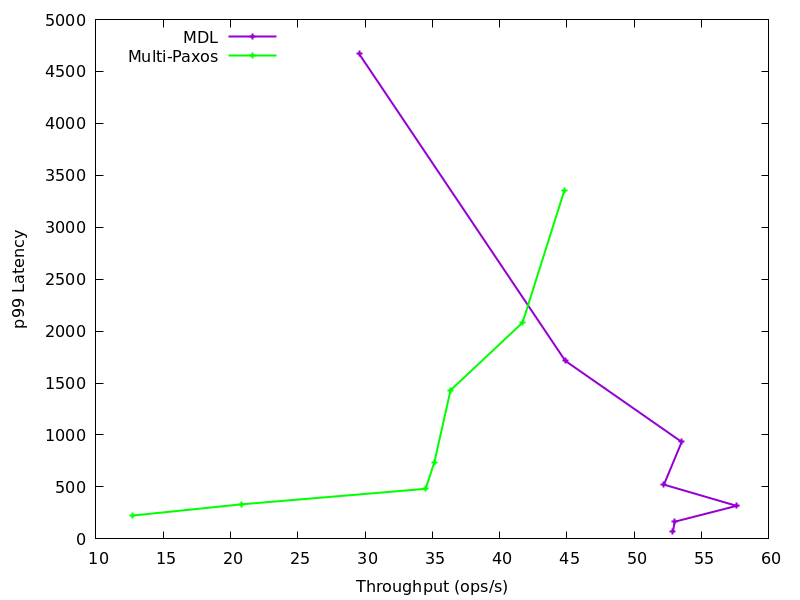
\includegraphics[scale=.15]{figs/1shard_fanout1000_p99.png}
}
\caption{p99 for single shard setting.}
\end{figure*}
%%%%%%%%%%%%%%%%%%%%%%%%%%%%%%%%%%%%%%%%
%%%%%%%% 1 shard uniform p50  %%%%%%%%%%
%%%%%%%%%%%%%%%%%%%%%%%%%%%%%%%%%%%%%%%%
\begin{figure*}[!htb]
\centering
\subfloat[Fanout\xspace1]{
  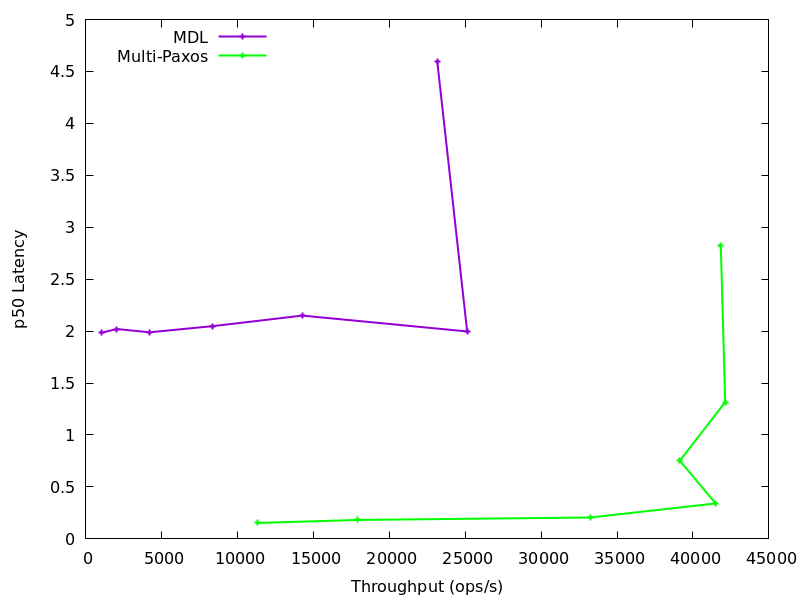
\includegraphics[scale=.15]{figs/1shard_fanout1_p50.png}
}
\subfloat[Fanout\xspace10]{
  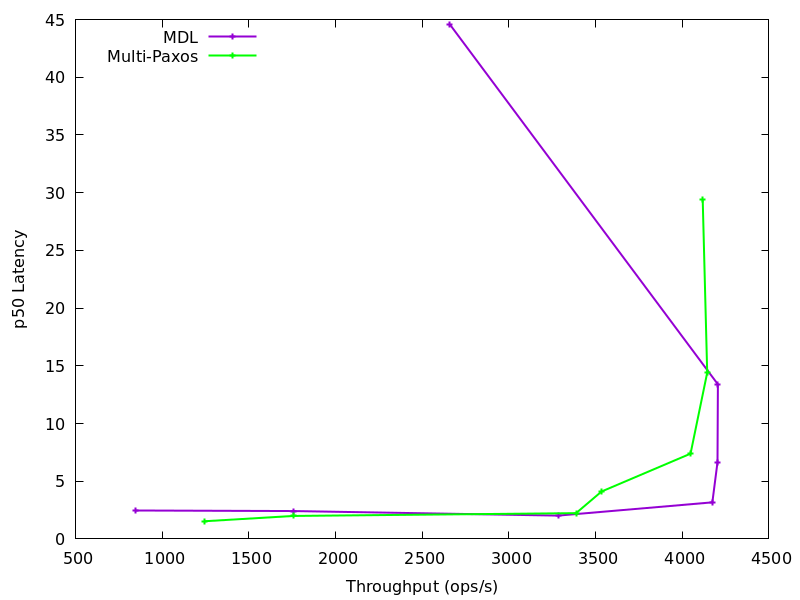
\includegraphics[scale=.15]{figs/1shard_fanout10_p50.png}
}
%\hspace{0mm}
\subfloat[Fanout\xspace100]{
  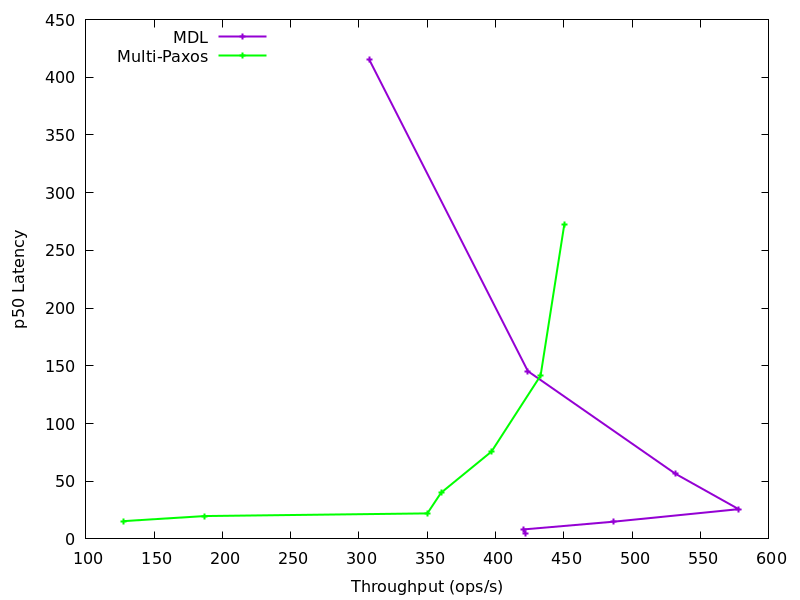
\includegraphics[scale=.15]{figs/1shard_fanout100_p50.png}
}
\subfloat[Fanout\xspace1000]{
  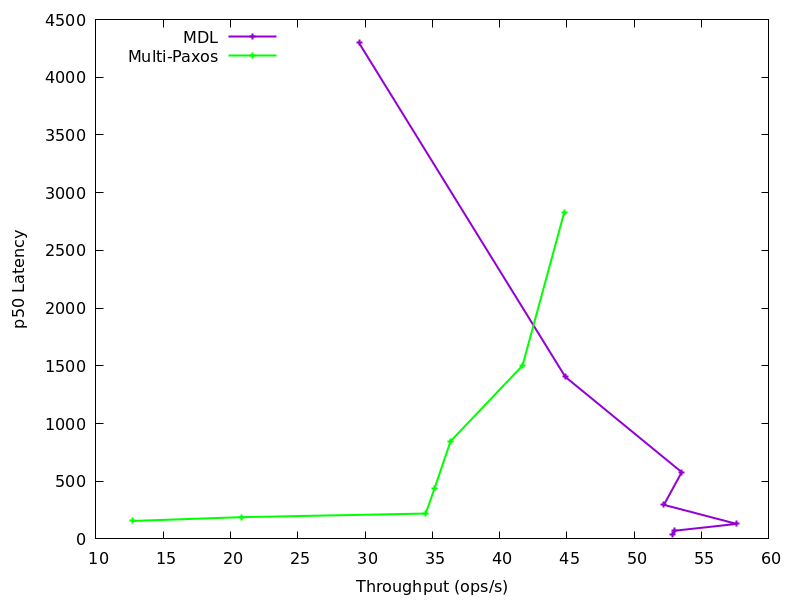
\includegraphics[scale=.15]{figs/1shard_fanout1000_p50.png}
}
\caption{p50 for single shard setting.}
\end{figure*}

%%%%%%%%%%%%%%%%%%%%%%%%%%%%%%%%%%%%%%%%%%%%%%%%%%%%%%%%%%%%%%%%%%%%%%%%%%%%%%%%%%%
%%%%%%%%%%%%%%%%%%%%%%%%%%%%%%%%%%%%%%%%%%%%%%%%%%%%%%%%%%%%%%%%%%%%%%%%%%%%%%%%%%%

%%%%%%%%%%%%%%%%%%%%%%%%%%%%%%%%%%%%%%%%
%%%%%%%% 3 shard uniform p99 %%%%%%%%%%%
%%%%%%%%%%%%%%%%%%%%%%%%%%%%%%%%%%%%%%%%
\begin{figure*}[!htb]
\centering
\subfloat[Fanout\xspace1]{
  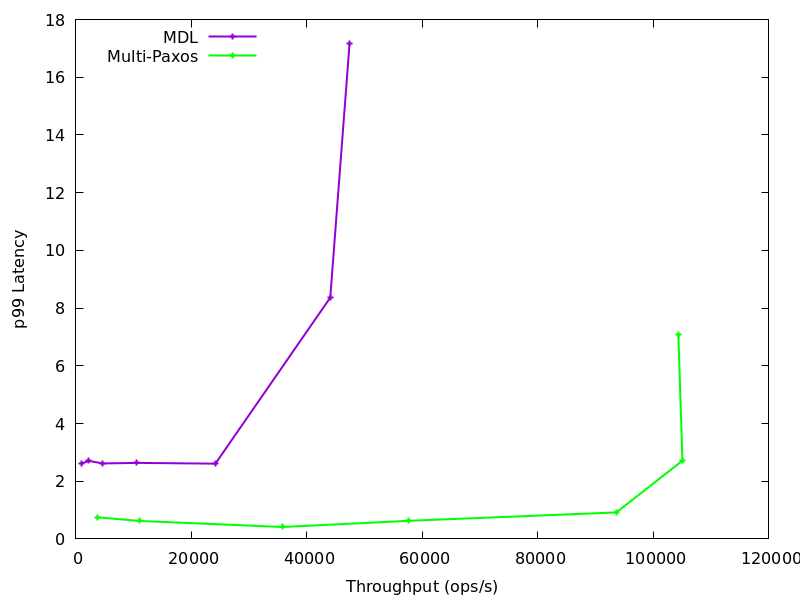
\includegraphics[scale=.15]{figs/3shard_fanout1_p99.png}
}
\subfloat[Fanout\xspace10]{
  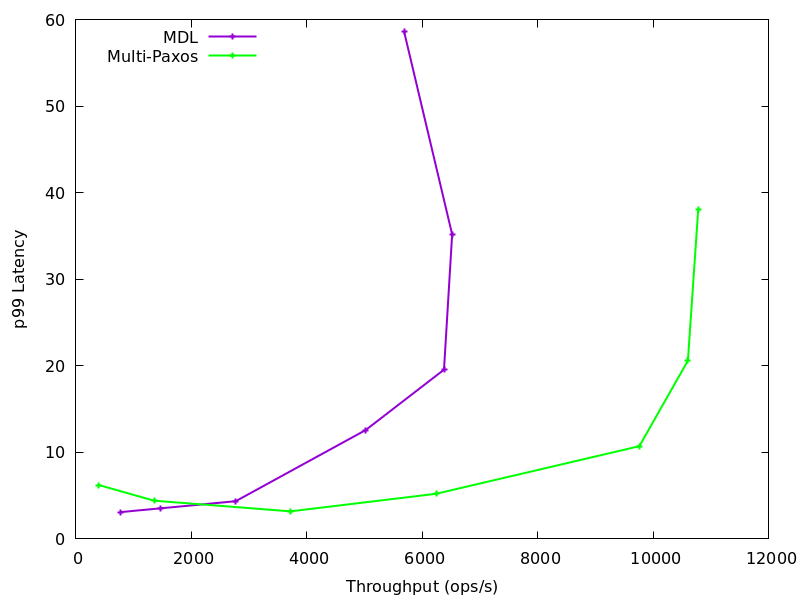
\includegraphics[scale=.15]{figs/3shard_fanout10_p99.png}
}
%\hspace{0mm}
\subfloat[Fanout\xspace100]{
  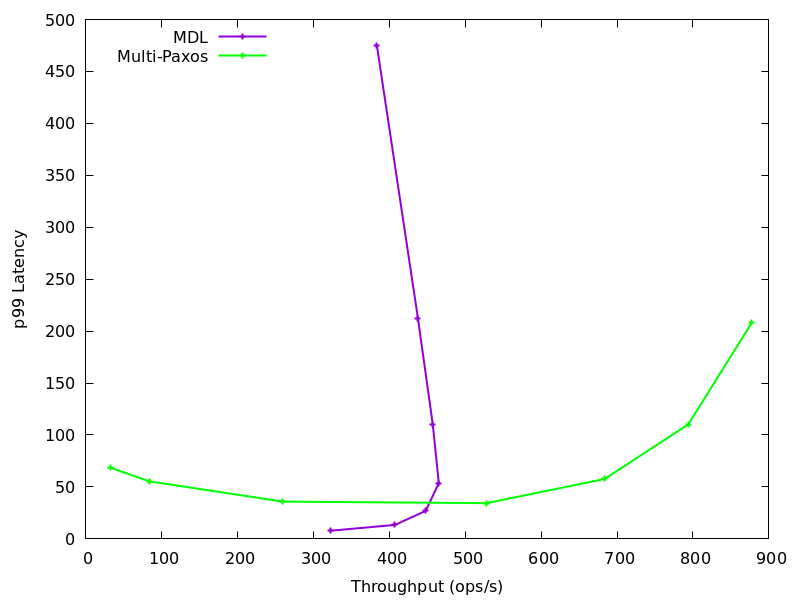
\includegraphics[scale=.15]{figs/3shard_fanout100_p99.png}
}
\subfloat[Fanout\xspace1000]{
  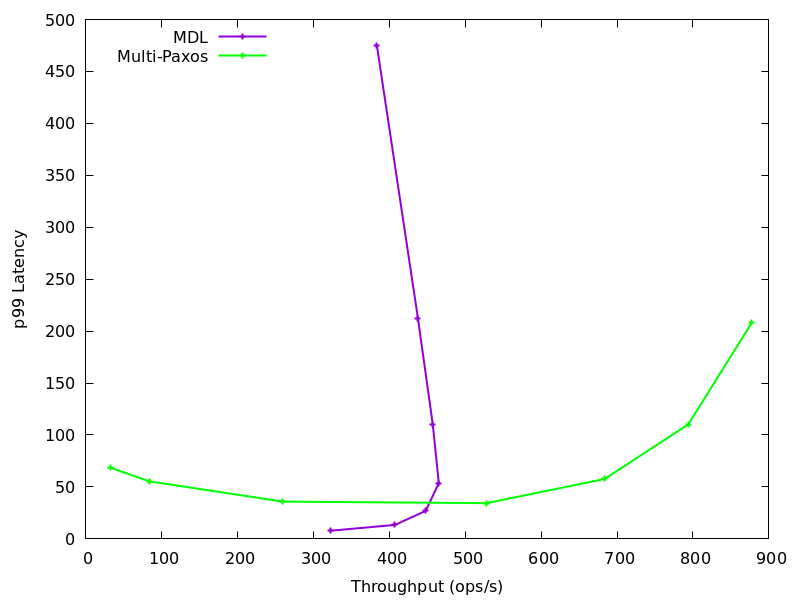
\includegraphics[scale=.15]{figs/3shard_fanout100_p99.png}
}
\caption{p99 for 3 shard setting.}
\end{figure*}

%%%%%%%%%%%%%%%%%%%%%%%%%%%%%%%%%%%%%%%%
%%%%%%%% 3 shard uniform p50  %%%%%%%%%%
%%%%%%%%%%%%%%%%%%%%%%%%%%%%%%%%%%%%%%%%
\begin{figure*}[!htb]
\centering
\subfloat[Fanout\xspace1]{
  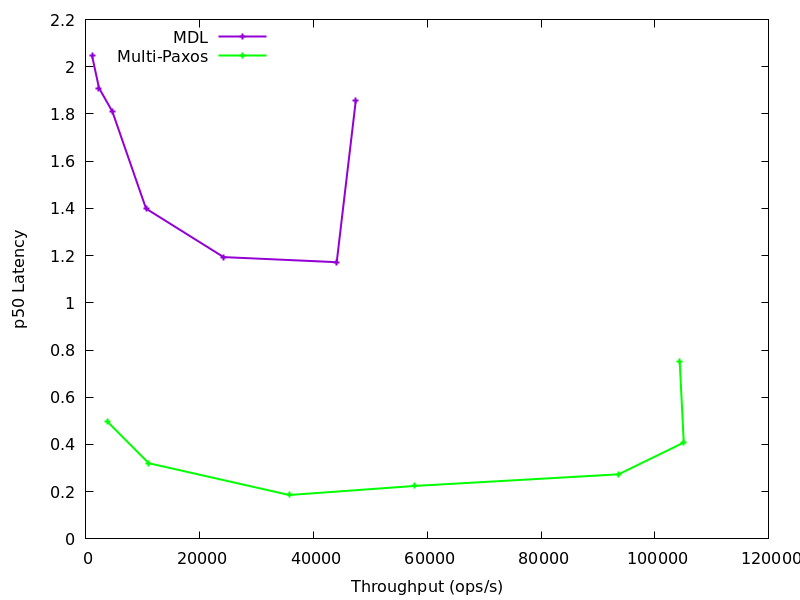
\includegraphics[scale=.15]{figs/3shard_fanout1_p50.png}
}
\subfloat[Fanout\xspace10]{
  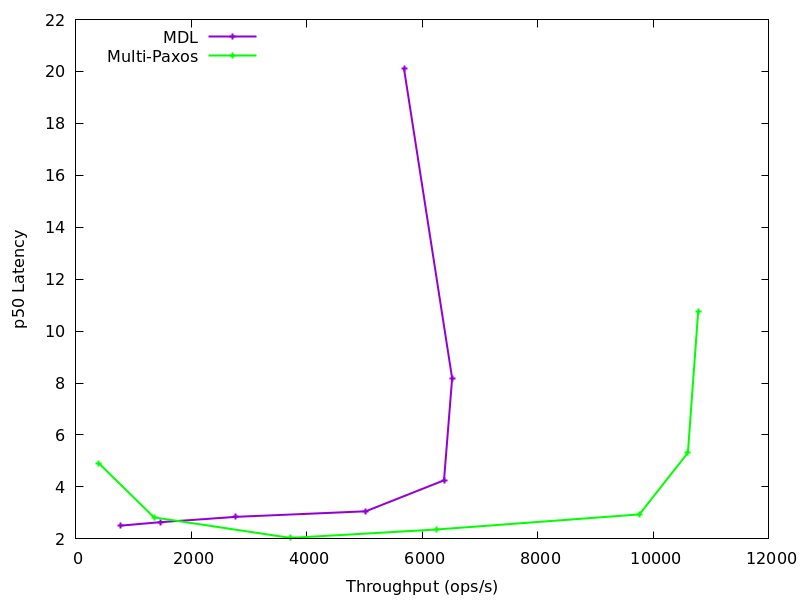
\includegraphics[scale=.15]{figs/3shard_fanout10_p50.png}
}
%\hspace{0mm}
\subfloat[Fanout\xspace100]{
  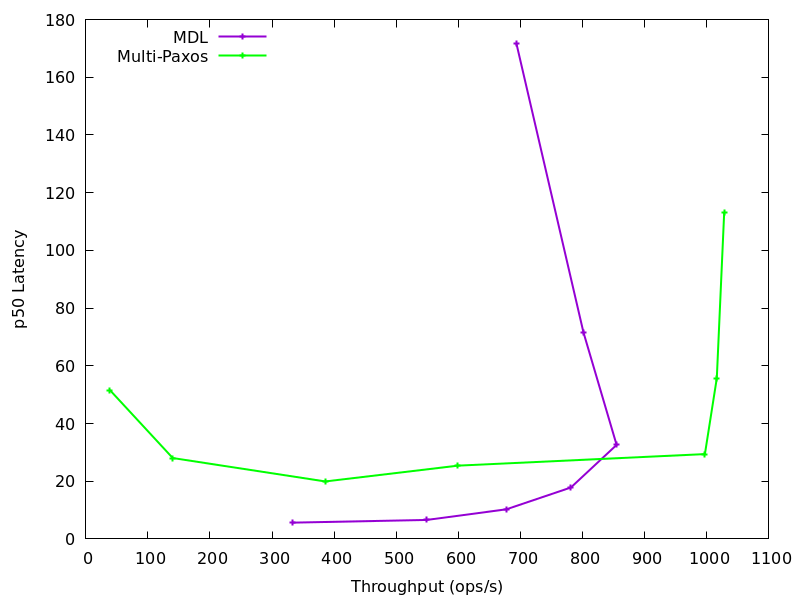
\includegraphics[scale=.15]{figs/3shard_fanout100_p50.png}
}
\subfloat[Fanout\xspace1000]{
  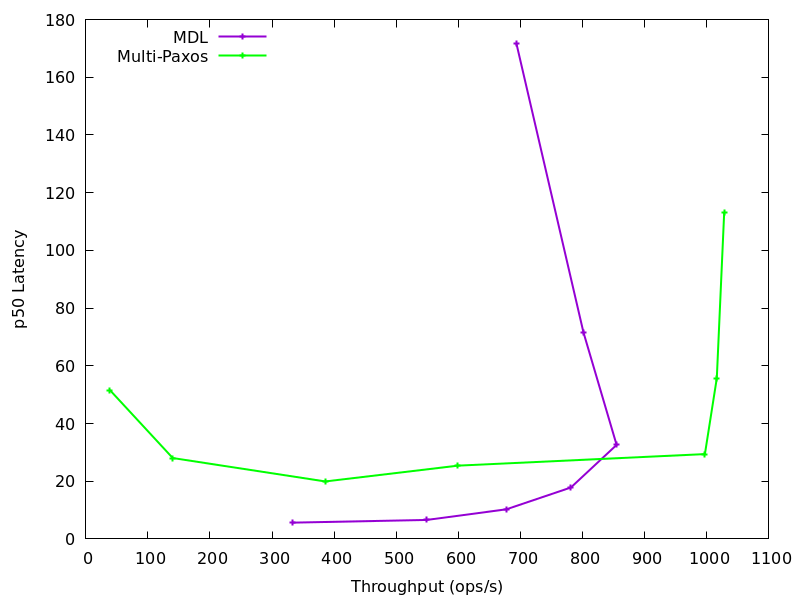
\includegraphics[scale=.15]{figs/3shard_fanout100_p50.png}
}
\caption{p50 for 3 shard setting.}
\end{figure*}


%%%%%%%%%%%%%%%%%%%%%%%%%%%%%%%%%%%%%%%%
%%%%%%%% 9 shard uniform p99 %%%%%%%%%%%
%%%%%%%%%%%%%%%%%%%%%%%%%%%%%%%%%%%%%%%%
\begin{figure*}[!htb]
\centering
\subfloat[Fanout\xspace1]{
  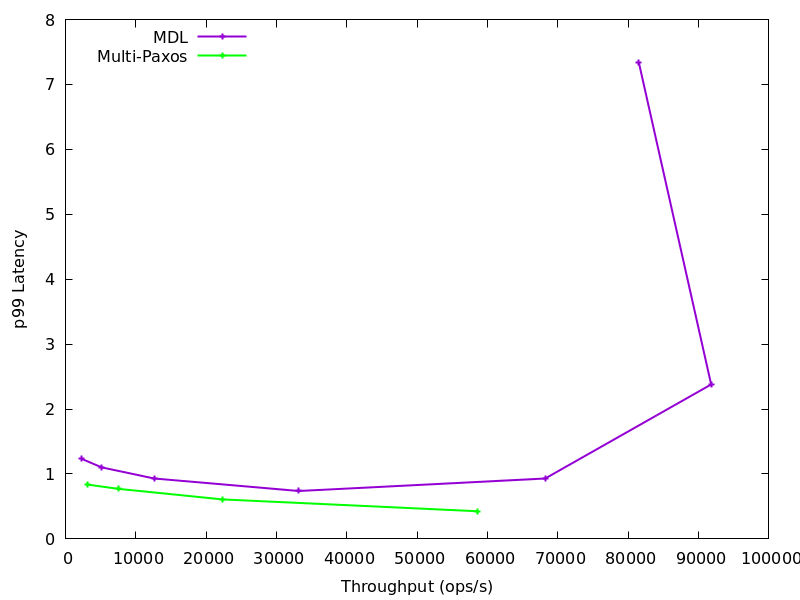
\includegraphics[scale=.15]{figs/9shard_fanout1_p99.png}
}
\subfloat[Fanout\xspace10]{
  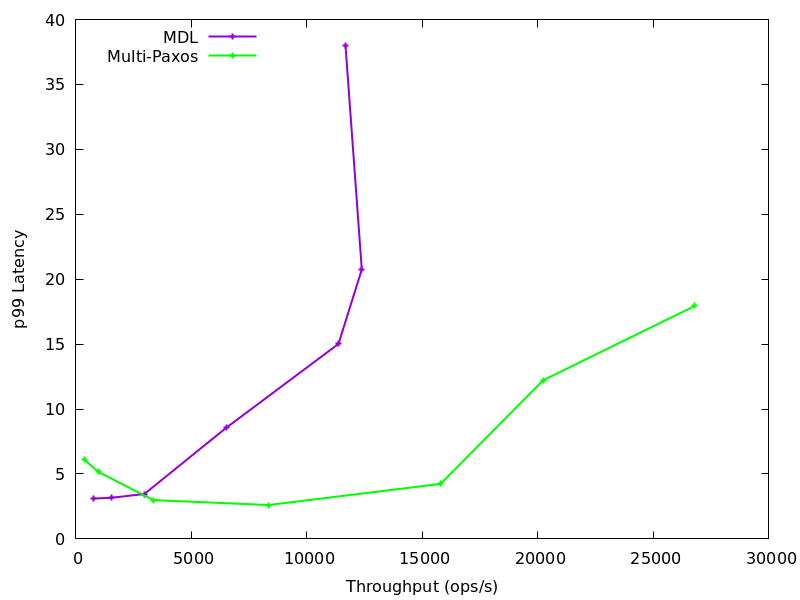
\includegraphics[scale=.15]{figs/9shard_fanout10_p99.png}
}
%\hspace{0mm}
\subfloat[Fanout\xspace100]{
  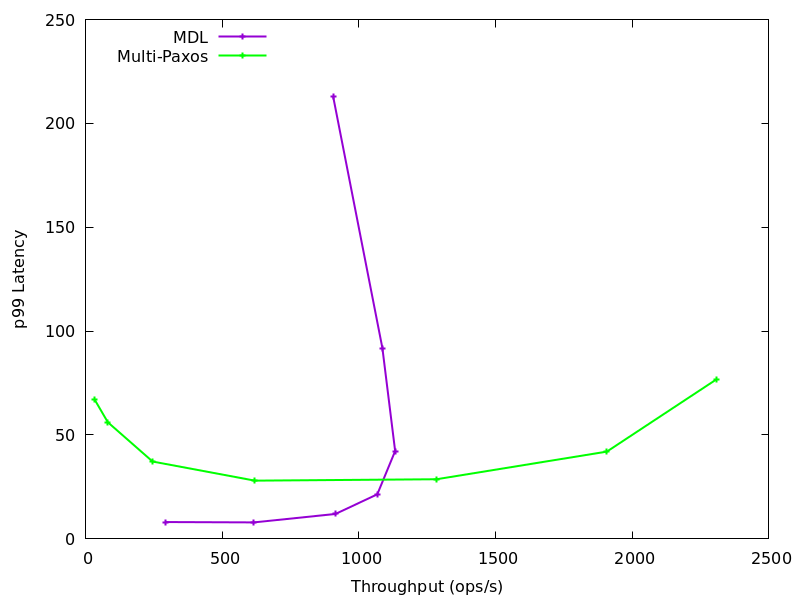
\includegraphics[scale=.15]{figs/9shard_fanout100_p99.png}
}
\subfloat[Fanout\xspace1000]{
  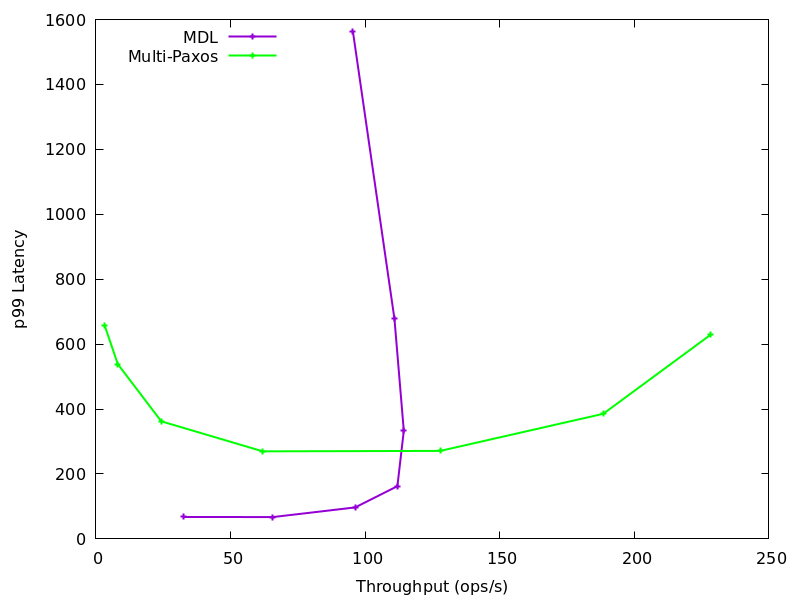
\includegraphics[scale=.15]{figs/9shard_fanout1000_p99.png}
}
\caption{p99 for 9 shard setting.}
\end{figure*}

%%%%%%%%%%%%%%%%%%%%%%%%%%%%%%%%%%%%%%%%
%%%%%%%% 9 shard uniform p50  %%%%%%%%%%
%%%%%%%%%%%%%%%%%%%%%%%%%%%%%%%%%%%%%%%%
\begin{figure*}[!htb]
\centering
\subfloat[Fanout\xspace1]{
  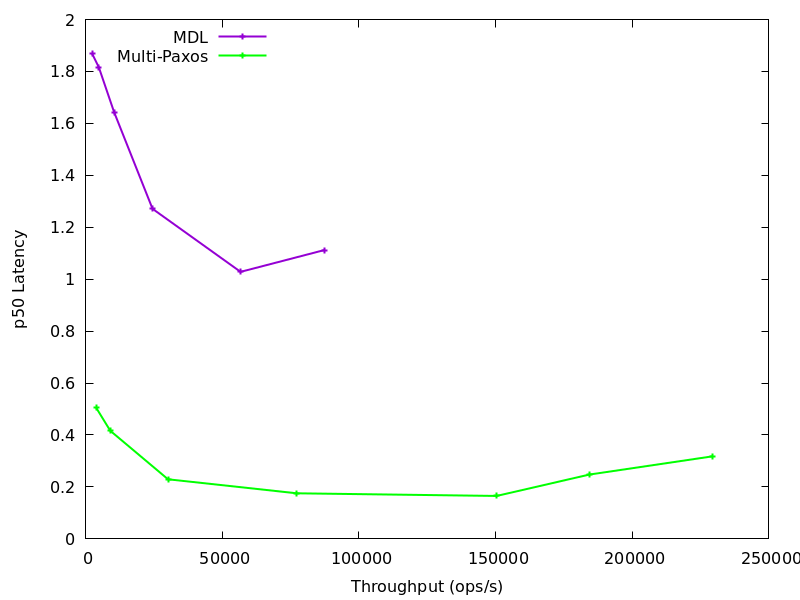
\includegraphics[scale=.15]{figs/9shard_fanout1_p50.png}
}
\subfloat[Fanout\xspace10]{
  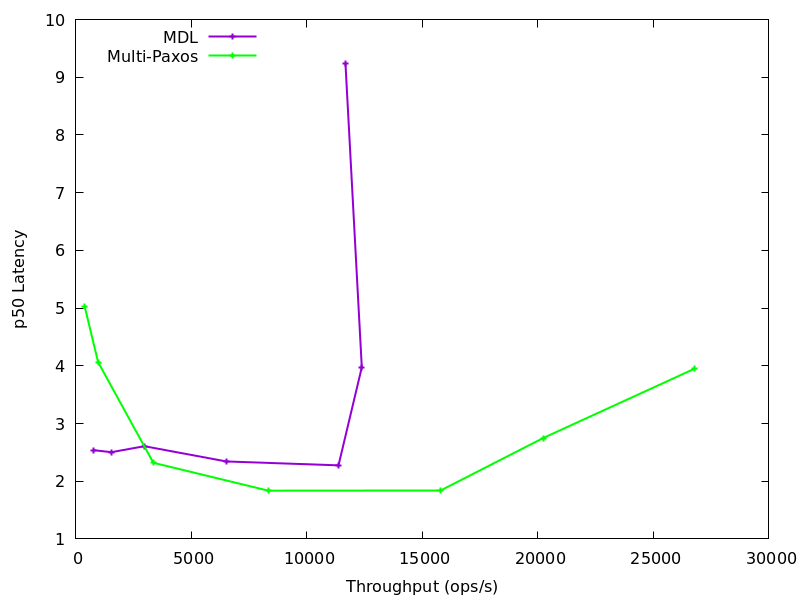
\includegraphics[scale=.15]{figs/9shard_fanout10_p50.png}
}
%\hspace{0mm}
\subfloat[Fanout\xspace100]{
  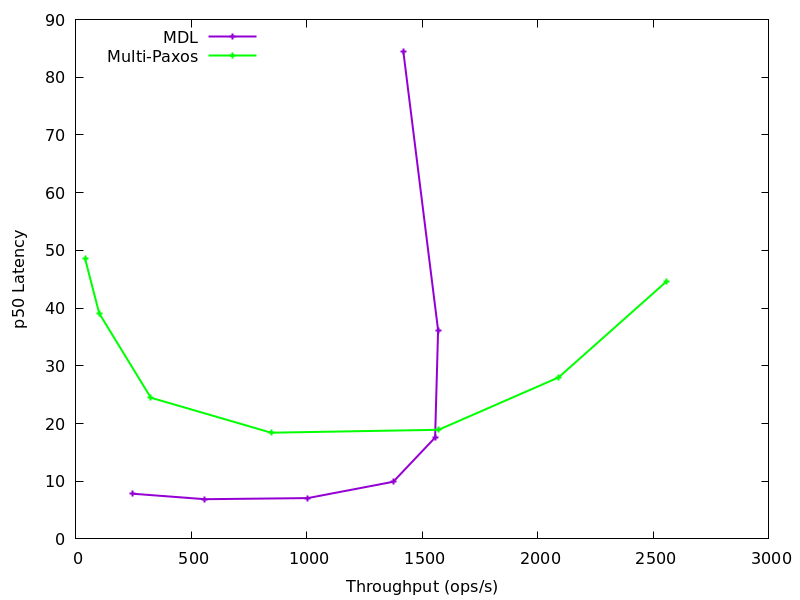
\includegraphics[scale=.15]{figs/9shard_fanout100_p50.png}
}
\subfloat[Fanout\xspace1000]{
  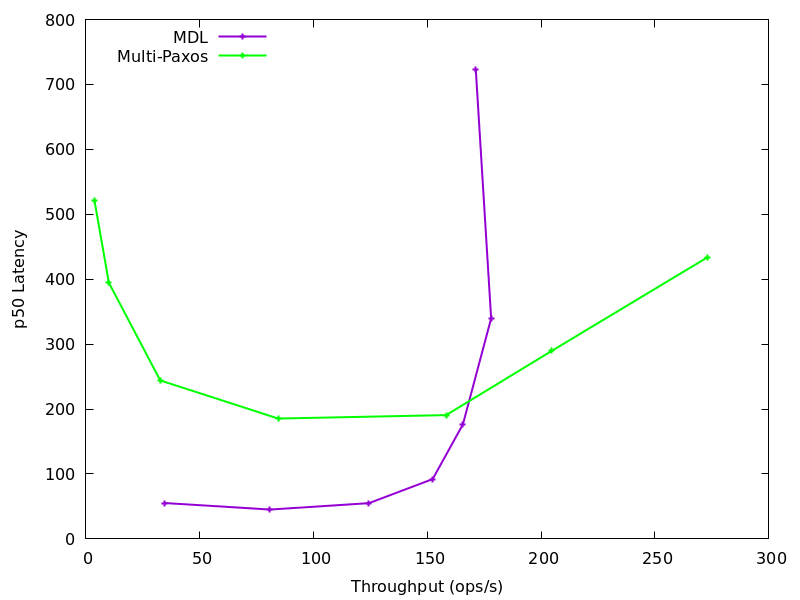
\includegraphics[scale=.15]{figs/9shard_fanout1000_p50.png}
}
\caption{p50 for 9 shard setting.}
\end{figure*}
%\end{comment}
%%%%%%%%%%%%%%%%%%%%%%%%%%%%%%%%%%%%%%%%%%%%%%%%%%%%%%%%%%%%%%%%%%%%%%%%%%%%%%%%%%%
%%%%%%%%%%%%%%%%%%%%%%%%%%%%%%%%%%%%%%%%%%%%%%%%%%%%%%%%%%%%%%%%%%%%%%%%%%%%%%%%%%%


